\documentclass{beamer}

\usepackage[utf8]{inputenc}
\usepackage{listings}
\usepackage{tikz}
\usepackage[style=alphabetic,giveninits=true,terseinits=true]{biblatex}

\definecolor{tumblue}{RGB}{0,101,189}
\definecolor{dkgreen}{rgb}{0,0.6,0}
\definecolor{mauve}{rgb}{0.58,0,0.82}
\lstset{
    basicstyle=\footnotesize\ttfamily,%
    columns=fullflexible,%
    keywordstyle=\bfseries\color{blue},%
    commentstyle=\color{dkgreen},%
    stringstyle=\color{mauve},%
}

\DeclareFieldFormat{url}{\href{#1}{\resizebox{!}{2ex}{\lower3pt\hbox{\pgfuseimage{beamericononline}}}}}

\setbeamerfont{footnote}{size=\tiny}
\renewcommand\footnoterule{}
\usecolortheme{orchid}
\setbeamertemplate{navigation symbols}{}
\setbeamertemplate{sidebar right}{% also implies no navbar
  \llap{\tikz\fill[tumblue,scale=.1] (0,0) ++(-5cm,-5cm) ++(-10cm,0)
      +(0cm,0cm) -- +(4cm,0cm) -- +(4cm,-4cm) -- +(5cm,-4cm) -- +(5cm,0cm) --
      +(10cm,0cm) -- +(10cm,-5cm) -- +(9cm,-5cm) -- +(9cm,-1cm) --
      +(8cm,-1cm) -- +(8cm,-5cm) -- +(7cm,-5cm) -- +(7cm,-1cm) --
      +(6cm,-1cm) -- +(6cm,-5cm) -- +(3cm,-5cm) -- +(3cm,-1cm) --
      +(2cm,-1cm) -- +(2cm,-5cm) -- +(1cm,-5cm) -- +(1cm,-1cm) --
      +(0cm,-1cm) -- cycle;}
  % Slide number in triangle.
  \vfill\llap{\tikz\path[fill=tumblue,inner sep=3pt] (0,0) -- ++(-1cm,0) -- +(1cm,1cm) -- cycle node[anchor=south east] {\usebeamerfont{footline}\color{white}\bfseries\insertframenumber};}%
  % Variant without triangle
  %\vfill\llap{\usebeamerfont{footline}\usebeamercolor[fg]{footline}\insertframenumber\hskip3pt}\vskip3pt%
}

\title{Transferring Hardware-related Information in sys-sage Across Processes and HPC Nodes}
\author{Finn Romanessen}
\institute{School of Computation, Information, and Technology\\Technical University of Munich}
\date{29.05.2024}

\renewcommand{\baselinestretch}{1.5}

\begin{document}

\begin{frame}
\titlepage
\end{frame}



\begin{frame}{Sys-Sage}
    \begin{itemize}
        \item Library to store and manage hardware topology information
        \item Designed to be highly dynamic and customizable
        \item Topologies consist of a component tree and DataPath graph
        \item Arbitrary data can be attached to components and DataPaths
    \end{itemize}
\end{frame}

\begin{frame}{Sys-Sage}
    \begin{figure}[!ht]
        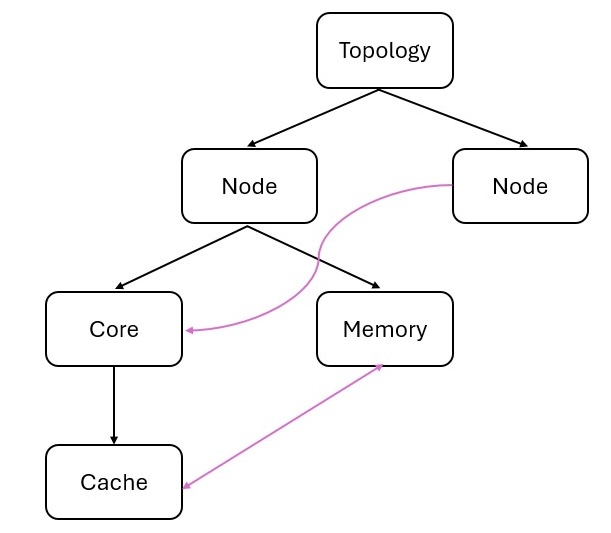
\includegraphics[scale=0.5]{../images/Topology_Example.jpg}
        \centering
    \end{figure}
\end{frame}

\begin{frame}{Motivation}
    \begin{itemize}
        \item Share sys-sage topologies between processes and nodes
        \item Hardware topologies within a HPC system are often very similar
        \item Share current information about the hardware state
    \end{itemize}
\end{frame}

\begin{frame}{Approach}
    \begin{itemize}
        \item Exporting process copies topology into shared memory
        \item All parts are arranged sequentially in the memory region
        \item Any process can import the topology by recreating it in local memory
    \end{itemize}
\end{frame}

\begin{frame}{Shared Memory}
    \begin{itemize}
        \item Shared memory regions created using memory-mapped files
        \item Virtual memory addresses different in each process
        \item Offset based pointers used within shared memory block
    \end{itemize}
\end{frame}

\begin{frame}{Components}
    \begin{itemize}
        \item Represent specific parts of the hardware
        \item Vectors have to be transformed to offset based implementation \lstinline|CopyVector|
        \item Pointers to children are replaced with offsets
    \end{itemize}
\end{frame}

\begin{frame}{Components}
    \begin{figure}[!ht]
        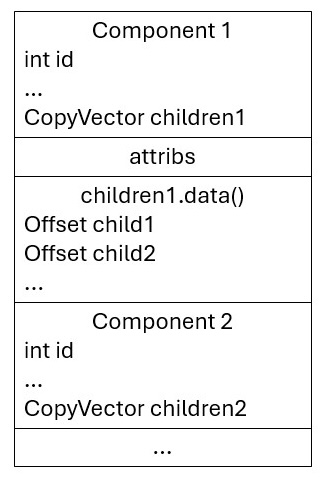
\includegraphics[scale=0.55]{../images/component_memory.jpg}
        \centering
    \end{figure}
\end{frame}

\begin{frame}{Attribs}
    \begin{itemize}
        \item Store arbitrary data in key-value map
        \item Data needs to be contiguous
        \item Map items are copied into sequential memory block
        \item Size and data supplied using \lstinline|pack()| function
    \end{itemize}
\end{frame}

\begin{frame}{Attribs}
    \begin{figure}[!ht]
        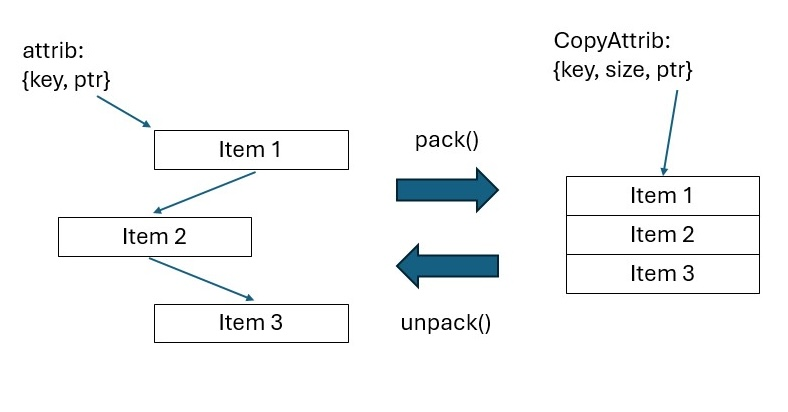
\includegraphics[scale=0.53]{../images/Slide4.jpg}
        \centering
    \end{figure}
\end{frame}

\begin{frame}{DataPaths}
    \begin{itemize}
        \item Represent relationships between components
        \item DataPaths are only exported if both components exported
        \item Offsets of source and target component in shared memory stored
    \end{itemize}
\end{frame}

\begin{frame}{DataPaths}
    \begin{figure}[!ht]
        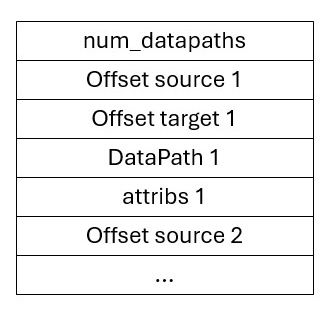
\includegraphics[scale=0.7]{../images/export_dps.jpg}
        \centering
    \end{figure}
\end{frame}

\begin{frame}{Performance}
    \begin{figure}[!ht]
        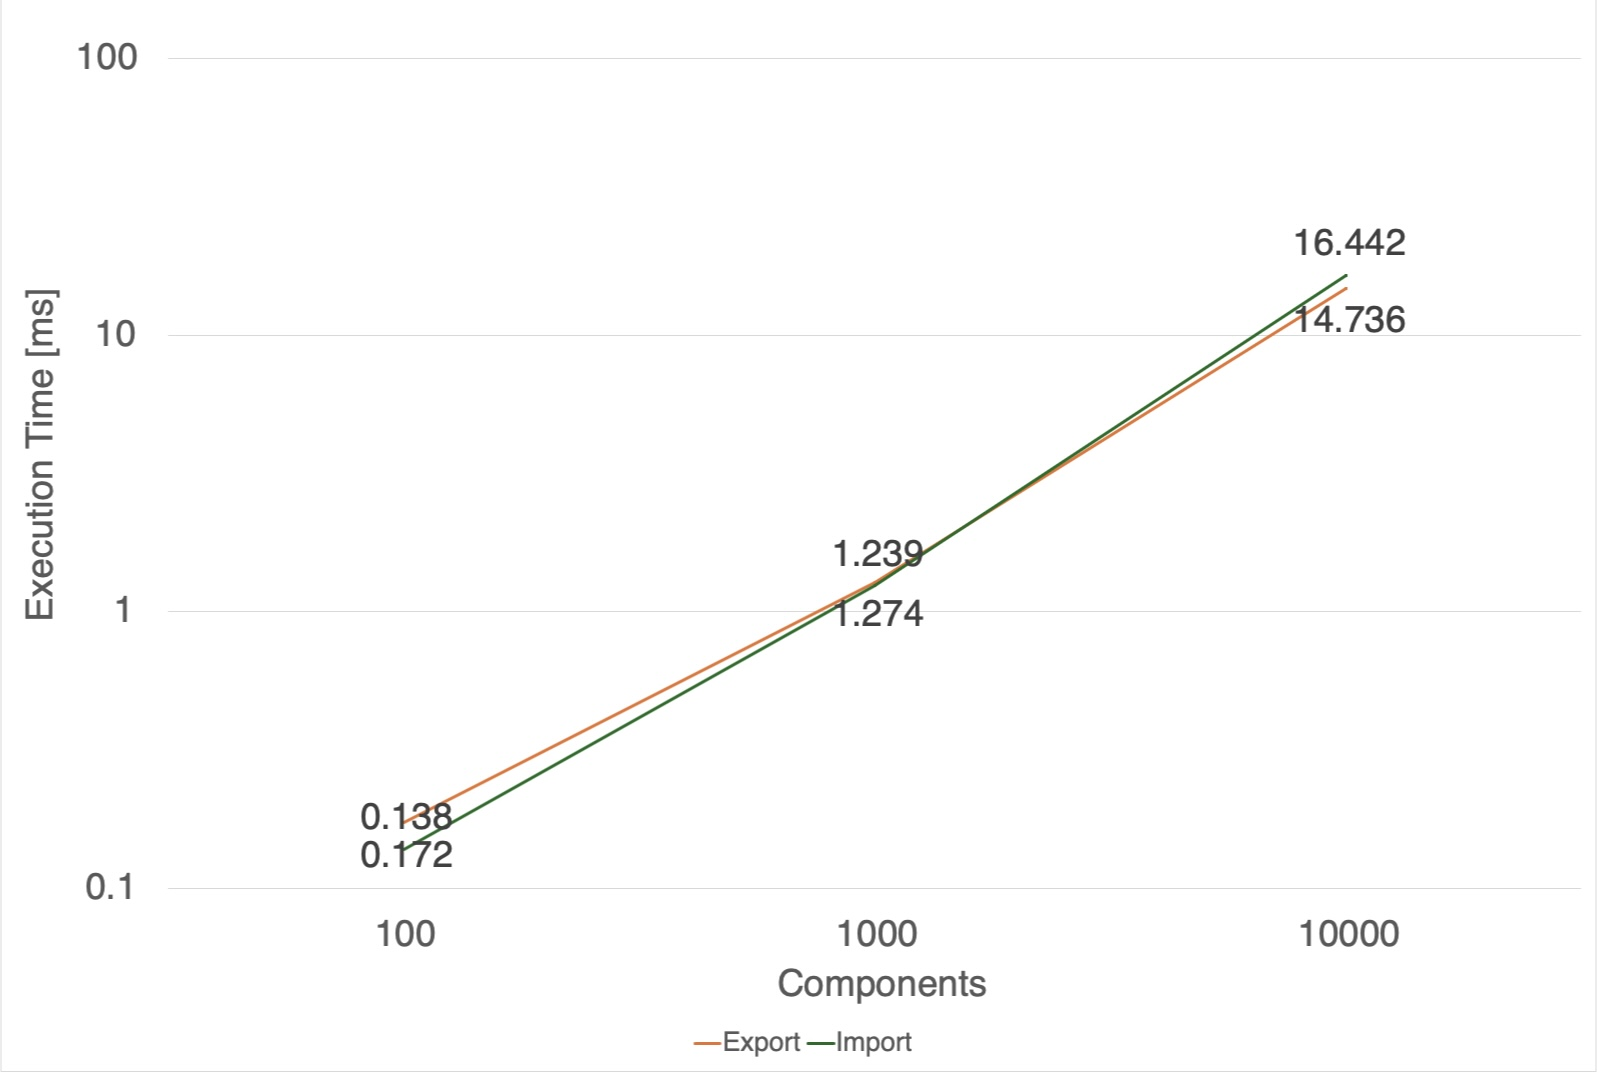
\includegraphics[scale=0.19]{../images/component_numbers.jpeg}
        \centering
    \end{figure}
\end{frame}

\begin{frame}{Future Work}
    \begin{itemize}
        \item Functionality to update existing shared topologies
        \item Make topologies usable within shared memory
        \item Changes possible from all processes
    \end{itemize}
\end{frame}

\begin{frame}{Conclusion}
    \begin{itemize}
        \item Share sys-sage topologies between processes and nodes
        \item Implementation uses memory-mapped files
        \item Topologies are deconstructed and reconstructed by importing process
    \end{itemize}
\end{frame}

\end{document}
